\chapter{Analysis of correctness and performance}
\label{ch:analysis}

Up to this point we described our system specification in detail.
Of course, specification alone does not establish any truths.
In this chapter, we evaluate our system analytically.
First we show it has the desired properties.
That is, the properties of the consensus protocol and the validation protocol (\Cref{def:consensus} and \Cref{def:validation} respectively) should hold.
Then we analyse the performance, especially the throughput,
and show that it out performs classical blockchain systems.
Finally, we consider the case where the $n \ge 3t + 1$ assumption is violated,
and show the effect of it in our system.

\section{Correctness in the presense of faults}
Our first objective is to show that \Cref{def:consensus} holds for our consensus protocol.
Then, building on top of it, we show \Cref{def:validation} holds for the validation protocol.
The resulting theorem shows that only using CP blocks in the consensus algorithm implies consensus on TX blocks.

% Our first objective in this section is to establish truths regarding the correctness of our protocol.
% We do this in two parts.
% First we use mathematical induction to show that properties in \Cref{def:consensus} holds for all round.
% Building on top that, if \Cref{def:consensus} is true, then we can show that many properties in \Cref{def:validation} is true.

\subsection{Correctness of the consensus protocol}

We begin our analysis by establishing truths on the four properties in \Cref{def:consensus},
namely agreement, validity, fairness and termination for an arbitrary round.
Using these results, we use mathematical induction to show that they hold for all rounds.

\begin{lemma}
\label{lemma:agreement}
For an arbitrary round $r$
if $\F_{r}$ is known by all correct nodes and one correct node outputs a list of facilitators $\F_{r+1}$,
then all correct nodes output $\F_{r+1}$.
\end{lemma}
\begin{proof}
The argument follows from the protocol description.
Given that $\F_r$ is known,
correct nodes will send CP blocks to all members in $\F_r$.
The ACS algorithm starts independently whenever the facilitator has $N - t$ valid CP blocks
(recall from \Cref{sec:consensus-phase} that invalid blocks are ones with an invalid signature or has a duplicate signature).
It cannot make progress until $n-t$ honest facilitators start algorithm,
but this eventually happens because there are $N - t$ correct nodes and all correct facilitator eventually receives $N -t$ valid CP blocks.
At the end of ACS, some $\C_{r+1}$ is created, and is broadcasted along with the signature of the facilitators.
Due to the agreement property of ACS (\Cref{def:acs}),
every correct node should receive at least $n - t$ valid signatures on the agreed $\C_{r+1}$.
Thus they use $\C_{r+1}$ to generate a new CP block and compute new facilitators.
Since $\textsf{get\_facilitators}(\cdot)$ is a deterministic algorithm and the input $\C_{r+1}$ is in agreement, the output $\F_{r+1}$ is also in agreement.
\end{proof}

\begin{lemma}
\label{lemma:validity}
For an arbitrary round $r$,
if $\F_r$ is known by all correct nodes and any correct node outputs $\F_{r+1}$,
then (a) $|\C_{r+1}| \ge N - t$ must hold for the $\C_{r+1}$ which was used to create $\F_{r+1}$,
(b) $\F_{r+1}$ must contain at least $n - t$ honest nodes and
(c) $|\F_{r+1}| = n$.
\end{lemma}
\begin{proof}
The validity follows from the validity property of ACS and the definition of our model,
namely $N \ge n + t$ and $n \ge 3t + 1$.
Given $\F_r$, since $N \ge n + t$ , there is at least $n$ nodes that would send their CP block to $\F_r$.
From the validity property of ACS, we know the output must contain the input of at least $n - 2t$ nodes.
But $n -t$ facilitators must have received $N - t$ valid CP blocks, so $|\C_{r+1}| \ge N-t$, this proves (a).
There are at least $n-t$ honest nodes in $\F_{r+1}$ which follows from our assumption, this proves (b).
Finally, since $N-t \ge (n+t) -t = n$ and $\textsf{get\_facilitators}(\cdot)$ outputs $n$ items, $|\F_{r+1}| = n$ and this proves (c).
\end{proof}

\begin{lemma}
\label{lemma:fairness}
For an arbitrary round $r$,
if $\F_r$ is known by all correct nodes then
every node with a CP block in $\C_{r+1}$, should have an equal probability to be elected as a facilitator in $\F_{r+1}$.
\end{lemma}
\begin{proof}
We already established that $|\C_{r+1}| \ge N - t \ge n$ from \Cref{lemma:validity}.
Then the proof directly follows from the random oracle model.
Recall that the luck value is computed using $\textsf{H}(\C_{r+1}, || pk_u)$.
Since $pk_u$ is unique for every node that has a CP block in $\C_{r+1}$,
the output of $\textsf{H}(\cdot)$ is uniformly random.
This effectively generates a random permutation
so every node has the same probability of being in the top $n$ for the ordered sequence,
namely the output of $\textsf{get\_facilitators}(\cdot)$.
\end{proof}

\begin{lemma}
\label{lemma:termination}
For an arbitrary round $r$,
if $\F_r$ is known by all correct nodes then
every correct node eventually outputs some $\F_{r + 1}$.
\end{lemma}
\begin{proof}
This follows directly from the properties of the channel (eventual delivery)
and the termination property of ACS.
That is, $\F_r$ eventually receives all the CP blocks required to begin ACS,
and then ACS eventually terminates.
Finally, the results are eventually dissemminated to all the nodes.
\end{proof}

From Lemmas \ref{lemma:agreement}, \ref{lemma:validity}, \ref{lemma:fairness} and \ref{lemma:termination},
we have shown that the 4 properties of \Cref{def:consensus} holds when assuming the existance of some $\F_r$.
Thus, to proof the whole of \Cref{def:consensus},
we need to proof these 4 properties under the universal quantifier.
We do this using mathematical induction.

\begin{theorem}
\label{theorem:consensus}
For all rounds,
the consensus protocol satisfies agreement, validity, fairness and termination (\Cref{def:consensus}).
\end{theorem}
\begin{proof}
We proof using mathematical induction.

In the base case ($r = 1$), agreement, validity fairness and termination follows directly from the bootstrap protocol.
Note that the result is $\F_1$, which indicates the facilitators that are agreed in round 1, who are responsible for driving the ACS protocol in round 2.

For the inductive step,
we assume that the 4 properties hold in round $r$ and prove that they also hold in round $r + 1$.
Using Lemmas \ref{lemma:agreement}, \ref{lemma:validity}, \ref{lemma:fairness} and \ref{lemma:termination},
it directly follows from modus ponens that these properties hold for $r + 1$.
Due to the principals of mathematical induction, these properties hold for all $r$.
\end{proof}

\subsection{Correctness of the validation protocol}
The consensus protocol (on CP blocks and facilitators) is the backbone for consensus on transactions.
In this section we build on top of \Cref{theorem:consensus} to show that the properties except liveness in \Cref{def:validation} can be satisfied.

\begin{theorem}
\label{theorem:validation-agreement}
% (Agreement of the validation protocol)
The validation protocol satisfies agreement and validity properties.
\end{theorem}
\begin{proof}
We proof the agreement property by contradiction.
Without loss of generality, suppose for some transaction with TX block $t$,
node $u$ decides \emph{valid} but node $v$ decides \emph{invalid}.
Then there exist a fragment $F' = \{ \dots, t', c'\}$ which $u$ received that contains a valid pair of $t$---$t'$.
There also exist a fragment $F'' = \{ \dots, t'', c''\}$ which $v$ received that does not contain or contains an invalid pair---$t''$.
In both cases, the $\textsf{get\_validity}(\cdot)$ function must have reached \Cref{line:valid-fragment}.
Due to \Cref{theorem:consensus}, we have $c' = c''$, otherwise the result would be \emph{unknown}.
Since $c' (= c'') = \langle \textsf{H}(t'), \dots \rangle$ we must have $\textsf{H}(t') = \textsf{H}(t'')$ and $t' \ne t''$ (because $t''$ is invalid).
In other words, the sender of $F''$ must be able to create some $t''$ that has the same digest as $t'$.
But this is only possible if the adversary can compute the inverse of $H(\cdot)$ with non-negligible probability.
Thus we have a contradiction and this completes the agreement proof.
Our protocol uses \Cref{alg:get-validity} which is also the validity definition,
this completes the validity proof.
\end{proof}

\Cref{theorem:validation-agreement} shows that agreement on CP blocks would lead to agreement on TX blocks when the nodes are running the validation protocol.
Just like in our prior work~\cite{implicitconsensus}, we call this behaviour implicit consensus.
One of the main advantages of our scheme over running a consensus algorithm on all the transactions is that 
the rate of transaction is no longer dependent on the consensus algorithm---ACS.
This enables horizontal scalability where adding new nodes would lead to higher global transaction rate.
In addition, a convenient consequence \Cref{theorem:validation-agreement} is unforgeability.
That is, no polynomial time adversary is able to create two chains $F = \{ \dots, t, c\}$ $F' = \{ \dots, t', c\}$ with correct hash pointers and the same end of chain $c$.
% Another way to think about it is if a transaction can be forged, then it cannot be agreed.

\subsection{Impossibility of liveness}
\Cref{theorem:validation-agreement} is a major result that allows significantly improved performance over traditional blockchain systems,
but it does not have all the properties of a typical Byzantine consensus protocol.
Now we show a negative result, where the liveness property of \Cref{def:validation} cannot be attained.
Meaning that trasanctions with adversaries cannot always be validated.

\begin{lemma}
There exist a valid transactions that cannot be validated eventually.
\end{lemma}
\begin{proof}
Suppose nodes $u$ and $v$ correctly perfomed the TX protocol which resulted a transaction.
Then when $u$ wants to validate it, it does so by sending \texttt{vd\_req} message to $v$.
$v$ can act maliciously and ignore all \texttt{vd\_req} message, then the transaction can never be validated.
\end{proof}
Although this is a negative result, it does not put the adversary in an advantageous position.
If the adversary is observed to ignore validation requests, then the honest nodes may prefer not to transact with her in the future.
Thus, to stay relevant in the system, the adversary need to comply to the protocol.

% \subsection{Chain structure}
% In this section we discuss how the adversary may tamper with the chain structure and its effects.
% The adversary can create invalid blocks, which are blocks that have an invalid hash pointer.
% The result is some chain with a broken link.

\section{Performance analysis}
\label{sec:performance-analysis}
This section aims to analytically answer the scalability aspect of our research question.
That is, does the global throughput increase linearly with respect to the population size?
We begin by looking at the communication and time complexity of the consensus protocol,
and then the bandwidth requirement for a single transaction.
We build on top of those results to analyse the global throughput.

\subsection{Communication complexity of the consensus protocol}
\label{sec:cons-complexity}
The consensus protocol can bee seen as three parts,
so the communication complexity is the sum of these parts.
The first part is when every node sends their CP block to all the facilitators, which is $O(Nn)$ since there are $N$ nodes and $n$ facilitators.
Or simply $O(N)$ if we consider $n$ as a constant.

The second part is ACS.
The communication complexity of ACS is $O(n^2|v| + \lambda n^3 \log n)$~\cite{miller2016honey},
where $|v|$ is the size of largest message and $\lambda$ is the security parameter (described in \Cref{sec:model-assumptions}).
In our system, we wish to understand the scalability property.
Thus we consider the complexity as a function of $N$ rather than $n$ or $\lambda$.
Since $|v|$ is at most all the CP blocks from every node, we have $|v| = kN$,
where $k$ is a constant representing the size of one CP block.
Therefore the communication complexity of ACS in our system is $O(N)$.
Since we use a constant $n$, $O(N)$ communication complexity also holds for a single facilitator.

% TODO wrong?
The third and final part is the dissemination, where the facilitators broadcast the consensus result along with their signatures.
For the same reason as the first part, this is also $O(N)$.
Thus the combined communication complexity when $n$ is a constant is $O(N)$.

% We argue that with a $O(N)$ message complexity we also have $O(N)$ time complexity.
% It is know that the running time is $O(\log n)$~\cite{miller2016honey}, which translates to $O(1)$ if our $n$ is constant.
% On the other hand, in many distributed algorithms, computational cost is small when compared to the communication cost.
% But in our system, we are more interested in the effect of the message size.

\subsection{Duration of the consensus protocol}
\label{sec:cons-duration}
In order to make arguments on bandwidth or throughput in our purely asynchronous model, which are concepts that depend on time,
we must make some assumptions regarding our model to make arguments on the duration of the consensus protocol.
Note that it is not the same as the time complexity typically used in distributed systems.
In analysis of distributed systems, time complexity is often in terms of the number of rounds.
For example, ACS runs in a constant number of rounds because its subprotocols---reliable broadcast and binary Byzantine consensus---also run in a constant number of rounds~\cite{miller2016honey}.
However, in practice, making a unit of communication always has some overhead associated with it, for example serialising and writing it to some network socket.
Hence, for the remainder of our performance analysis, we add the following to our computational model.
For every unit of communication, we assume they take some non-negligible but constant time to perform.
Hence, from~\Cref{sec:cons-complexity} and the fact that the consensus protocol uses a constant number of rounds,
it follows that the consensus protocol has a duration of $O(N)$.

\subsection{Communication cost for transactions}
\label{sec:communication-cost-for-tx}
With the analysis on the duration of the consensus protocol,
we are ready to analyse the amount of data required to be transmitted over a link per transaction,
which we call the communication cost per transaction.
% First, we define bandwidth as the ``amount of data a link or network path can deliver per unit of
% time''~\cite{prasad2003bandwidth}.
To create and then validate a transaction,
the communication cost per transaction is of $O(l)$,
where $l$ is the length of the agreed fragment.
This can be seen from the fact that the largest message by far is the \texttt{vd\_resp} message,
which contains the agreed fragment.
The other messages (\texttt{tx\_req}, \texttt{tx\_resp} and \texttt{vd\_req}) are constant factors.
If we assume that every node performs transactions at a constant rate of $r_{\text{tx}}$ per second.
Then
$$l = r_{\text{tx}} D_{\text{c}},$$
where $D_{\text{c}}$ is the duration a round of the consensus protocol.
But from \Cref{sec:cons-duration},
we know that $D_{\text{c}}$ is of $O(N)$, thus the communication cost per transaction is $O(N)$.
This is intuitive because round duration would be longer if there are more CP blocks (more $N$), which means that the agreed fragments are longer (assuming nodes transact at a constant rate).
The behaviour is verified experimentally in \Cref{ch:implementation}.

\subsection{Linear global throughput}
\label{sec:global-throughput}
Using our results so far, we are able to analyse the global throughput.
First we clarify the bandwidth definition, which is ``the data rate at which a network link or a network path can transfer''~\cite{prasad2003bandwidth}.
Now, suppose every node has some fixed bandwidth $C$ per link, $N$ links and are making transactions at $r_{\text{tx}}$ per second.
Then we have the inequality
$$NC \ge r_{\text{tx}} l,$$
where $l$ is the length of the the agree fragment as before.
The inequality suggests that the rate for which transactions and validations are made cannot exceed the total bandwidth of all the links.

We note that the inequality does not hold if the node is only transacting with a subset of the population.
This is because it cannot use all the bandwidth available in all the links.
In the extreme case, if the node is only transacting with one other node, then it can only use the bandwidth of one link which is only $C$.
However, if that is the case, we can intelligently cache the \texttt{vd\_resp} messages as described in~\Cref{sec:caching}.
For this work, we analyse the worst case where every node transacts with a random node from the population,
and a new \texttt{vd\_resp} must be sent for every \texttt{vd\_req} message.

Consider the case where the system is making use of all the bandwidth, i.e. $NC = r_{\text{tx}} l$.
Recall that $l$ is of $O(N)$, that means LHS and RHS both grow linearly with respect to $N$.
Hence, there exist some constant $r_\text{tx}$ that makes use of all the available bandwidth regardless of $N$.
Finally, if every node in the network is transacting at a constant rate, then the global throughput (in terms of transactions per second) is linear w.r.t. the population size $N$.
If the system is not making use of all the bandwidth.
We also maintain a constant transaction rate by the same argument.
Thus a global throughput is also linear w.r.t. $N$.
We verify both of these claims experimentally in~\Cref{ch:implementation}.

% The upshot of this analysis is that our system scales nicely at a global throughput of $O(N)$ until the population gets too large.
% Then we maintain a constant global throughput.
% This result falls a bit short of what we envisioned in the introduction.
% However, the population is not the number of nodes that use the system, but the number of nodes that are online during a single round.
% Furthermore, this result is for the worst case where every transaction needs an agreed fragment to be transmitted.
% In practice, nodes are able to cache agreed fragments.
% For instance, if $u$ and $v$ make $x$ transactions in a single round,
% then only one agreed fragment need to be exchanged as it contains all the transactions rather than $x$ agreed fragments.

\section{Effect of a highly adverserial environment}

Our last study consideres the effect when the number of adversaries is more than $t$.
This is useful because in practice it is difficult to guarantee that $t$ satisfied $n \ge 3t + 1$, especially when $N$ is large.
Hence we are interested in the probability for this to happen under our facilitator election process.

The problem can be formulated as follows.
Suppose an urn contains $N$ balls, $t$ are black (malicious) and $N-t$ are white (honest).
If $n$ balls are drawn uniformly at random without replacement,
what is the probability that more than $\lfloor \frac{n-1}{3} \rfloor$ are black?
The random variable $X$ in this case is the number of black balls, or the number of successful events.
It follows the hypergeometric distribution since we pick balls \emph{without} replacement~\cite{skala2013hypergeometric}.
Hence, we are interested in the following probability.
$$
1 - \sum_{k = 0}^{\lfloor \frac{n-1}{3} \rfloor} \Pr[X = k] = 
1 - \sum_{k = 0}^{\lfloor \frac{n-1}{3} \rfloor} \frac{ \binom{t}{k} \binom{N-t}{n-k} }{ \binom{N}{n} }
$$

This is not in closed form,
but we can visualise the effect in \Cref{fig:hypergeometric}.
We set the population size $N$ to 2000
and plot the probability of more than $\lfloor \frac{n-1}{3} \rfloor$ successful events for different numbers of draws.
Evidently,
if the number of black balls (traitors) is a third of the population (666 out of 2000)
we have about 0.5 probability of electing more than $\lfloor \frac{n-1}{3} \rfloor$ black balls for sufficiently large $n$.
Thus, we cannot expect the system to function correctly when 
the expected value is close to the number of black balls that we can tolerate.

\begin{figure}[h]
  \centering
  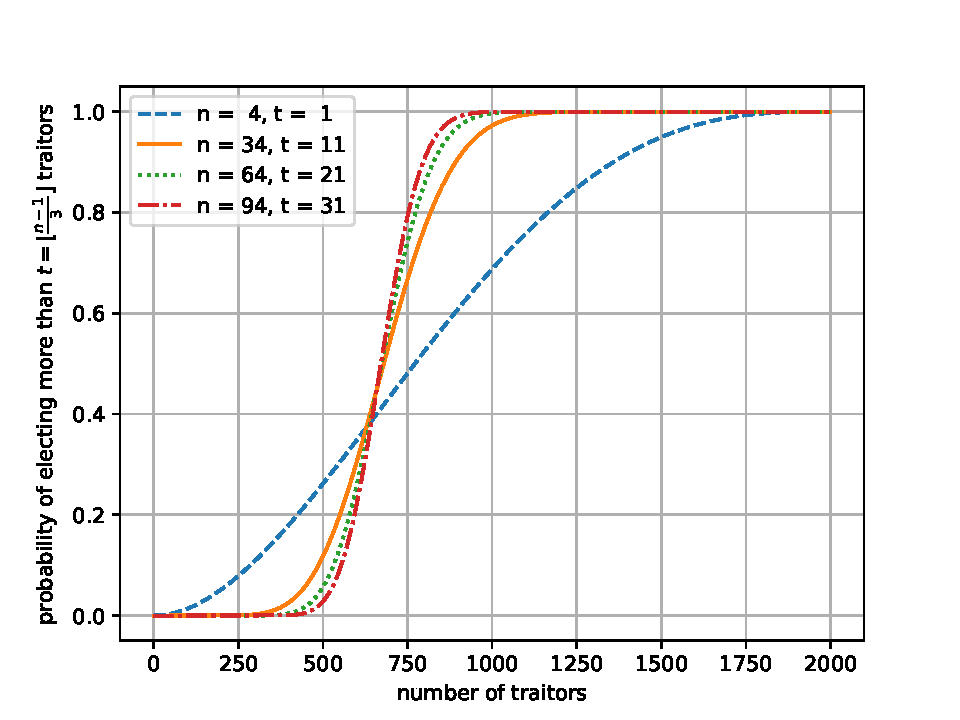
\includegraphics[width=1.0\textwidth]{hypergeometric}
  \caption{Plot of the probability of selecting more than $\lfloor \frac{n-1}{3} \rfloor$ black balls for
  different value of $t$ with $N$ fixed at 2000.}
  \label{fig:hypergeometric}
\end{figure}

On the other hand, due to the fact that hypergeometric distributions have light tails with ``faster-than-exponential fall-off''~\cite{skala2013hypergeometric},
the probability for picking more than $\lfloor \frac{n-1}{3} \rfloor$ black balls when 
the expected value is much smaller than $\lfloor \frac{n-1}{3} \rfloor$ is small.
We can use tail inequality to bound the probability of picking more than $\lfloor \frac{n-1}{3} \rfloor$ black balls when only $n\alpha$ are black where $0 \le \alpha \le \lfloor \frac{n-1}{3} \rfloor / n$.
The tail inequality is
$$
\Pr[X \ge E[X] + \tau n] \le e^{-2\tau^2n},
$$
where $E[X] = n\alpha$.
We are interested in $\Pr[X \ge \lfloor \frac{n-1}{3} \rfloor + 1]$, so
\begin{align*}
\tau &= \frac{\lfloor \frac{n-1}{3} \rfloor + 1}{n} - \alpha
\end{align*}
Putting $\tau$ back into the tail inequality we get the following bound.
$$
\Pr[X \ge \lfloor \frac{n-1}{3} \rfloor + 1] \le e^{-2 \big(\frac{\lfloor  \frac{n - 1}{3} \rfloor + 1}{n} - \alpha \big)^2 n}
$$

The bound is not tight, but it is useful for for picking parameters.
For some fixed $n$, since $0 \le \alpha \le \lfloor \frac{n-1}{3} \rfloor/n < (\lfloor  \frac{n - 1}{3} \rfloor + 1) / n$,
the probability is maximum when the squared term is minimum at $\alpha = \lfloor \frac{n-1}{3} \rfloor/n$.
The probability is minimum when the squared term is maximum at $\alpha = 0$.
Hence, if $n$ is known, then we can pick a $\alpha$ such that the probability becomes small.
On the other hand, if $\alpha$ is fixed, but small, we may increase $n$ to achieve the same.
To put this into perspective, suppose $n = 1000$ and $\alpha = 1/20$, then the probability to draw more black balls than the threshold is only $2 \times 10^{-48}$.

